\subsection{Safety Assessment Process}
\label{subsec:process}
ARP4754A, the Guidelines for Development of Civil Aircraft and Systems \cite{SAE:ARP4754A}, has been recognized by the Federal Aviation Administration (FAA) as an ``acceptable method for establishing a development assurance process'' \cite{AC:20-174}. It provides guidance on applying development assurance at each hierarchical level throughout the development lifecycle of highly-integrated/complex aircraft systems.

%Figure~\ref{fig:arp4754a_process} from [ref. ARP4754A] demonstrates the ARP4754A process flow. 
The safety assessment process is a starting point at each hierarchical level of the development lifecycle, and is tightly coupled with the system development and verification processes. It is used to show compliance with certification requirements, and meeting a company's internal safety standards \cite{SAE:ARP4754A}. ARP4761, the Guidelines and Methods for Conducting Safety Assessment Process on Civil Airborne Systems and Equipment \cite{SAE:ARP4761}, identifies a systematic means to show compliance. The guidelines presented in ARP4761 include industry accepted safety assessment processes (Functional Hazard Assessment (FHA), Preliminary System Safety Assessment (PSSA), and System Safety Assessment (SSA)), and safety analysis methods to conduct the safety assessment, such as Fault Tree Analysis (FTA), Failure Modes and Effect Analysis (FMEA), and Common Cause Analysis (CCA). 

\begin{comment}
\begin{figure}[h!]
	\vspace{-0.19in}
	\begin{center}
		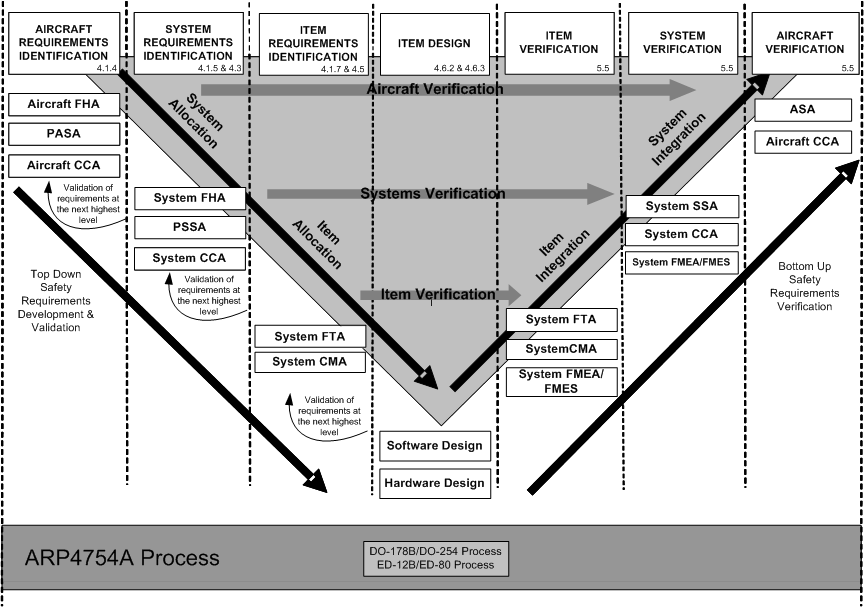
\includegraphics[trim=0 9 0 5,clip,width=1.0\textwidth]{images/ARP4754A_Process.png}
	\end{center}
	%\vspace{0.4in}
	\caption{ARP4754A Process(from ARP4754A ref)}
	\label{fig:arp4754a_process}
\end{figure}
\end{comment}

\begin{figure}[h!]
	\vspace{-0.19in}
	\begin{center}
		\includegraphics[trim=0 9 0 5,clip,width=0.9\textwidth]{images/Safety_Assessment_Process_update.png}
	\end{center}
	%\vspace{0.4in}
	\caption{Using the Shared System/Safety Model in the ARP4754A Safety Assessment Process}
	\label{fig:proposed_safety_process}
\end{figure}

A prerequisite of performing the safety assessment of a system design is to understand how the system works, primarily focusing on the integrity of the outputs and the availability of the product. The safety engineers then use the acquired understanding to construct the safety analysis artifacts, conduct safety analysis, and compare the analysis results with established safety objectives and safety related requirements. 

In practice, prior to performing the safety assessment of a system, the safety engineers are often equipped with fair amount of knowledge on how system works in general, but not necessarily with the specific system. Acquiring the knowledge on the content and behavior of a specific system has shown to be time consuming to get it right. In one real case example, it took a safety engineer two solid days to understand how the software works in a Stall Warning System (a small system in comparison to a flight control computer). The primary task includes threading the signal and function flows to relate the input and output signals from end-to-end, and understanding the causal effect between them. This is the same amount of time, if not more, as constructing the analysis artifacts and performing the analysis itself. In another real case example, it took a safety engineer almost a year to finalize the PSSA document for a Horizontal Stabilizer Control System (a medium system in comparison to a flight control computer), involving two major revisions and multiple rounds of reviews with system, hardware, and software engineers.

Capturing failure mode in models and generating safety analysis artifacts directly from models can enhance communication and synchronization between system design process and safety assessment process, and the ability to analyze complex systems. Industry practitioners have come to realize the benefits and importance of
using models to assist the safety assessment process (either by augmenting the existing system design model, or by building a separate safety model), and a revision of the ARP4761 with model based safety analysis appendix is under way.

Using the same system design model to conduct both system design and safety analysis can help reduce the gap in comprehending the system behavior and transferring the knowledge between the design model to the safety analysis model. It maintains a living model that captures the latest state of the system design as the process flows per the system development lifecycle.
%Figure~\ref{fig:arp4754a_process}. 
It also allows all participants of the ARP4754A process to be able to communicate and review the system design using the ``single source of truth''.

\begin{figure}[h!]
	\vspace{-0.19in}
	\begin{center}
		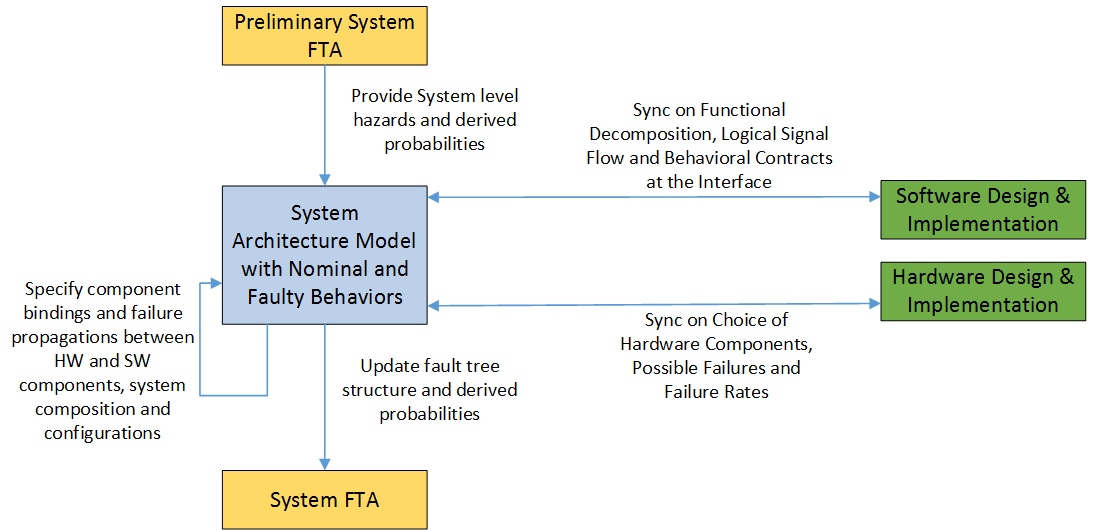
\includegraphics[width=0.9\textwidth]{images/FTA_MBD_Workflow.png}
	\end{center}
	%\vspace{0.4in}
	\caption{Example Interactions between the Shared System/Safety Model and  the FTAs}
	\label{fig:interaction_with_FTA}
\end{figure}

In order to allow performing system design and safety analysis on the same model, the system design model will need to be augmented to include both the system design information (e.g., system architecture, functional behavior) and safety-relevant information (e.g., failure mode, failure rate), at the same time keeping the two types of information distinguishable yet interactable from each other.

Figure~\ref{fig:proposed_safety_process} presents our proposed use of the shared system design and safety analysis model (to be referred as "the shared model" in the rest of this section) inside the ARP4754A Safety Assessment Process Model (Figure 7 of \cite{SAE:ARP4754A}). As seen in the figure, the shared model represents a system development artifact from the ``Development of System Architecture'' and ``Allocation of System Requirements to Item'' activities in the System Development Process, which interacts with the PSSAs and SSAs activities in the Safety Assessment Process. The shared model can serve as a wrapper and interface to capture the information relevant to safety analysis from the system design and implementation.

Figure~\ref{fig:interaction_with_FTA} shows an example how the preliminary FTAs and FTAs (artifacts from the PSSA and SSA activities in the Safety Assessment Process) can guide and be updated from the shared model. The next subsection will describe the foundation of the modeling technique in more details.

\begin{comment}
%check Figure 7 of ARP-4754A for step by step process of the traditional approach
%How our approach can help: step by step process; inputs and outputs
%Drawback/inefficiencies with the current safety assessment
%The causal effect in the fault tree is manually come up by safety engineers after understanding the signal and function flow in the system/sw design documents for the related functionality. 
%The logical causal relationship is represented in a descriptive fault tree structure. 
%It works well when the signals are processed in a sequential/linear fashion, but not when there are interactions/feedback loops that make the causal effect no longer linear?

%case study
%AIR6110, Rockwell white paper
"working on safety analysis process. Strategy:
1. Check the example Mike Peterson did with stall warning
2. Come up with model in our end
3. See if we can catch anything missed by the fault tree, or help supply the fault tree analysis"
start process investigation by:
1. select the example from stall warning where mike has produced a fault tree from the document
2. independently model from the stall warning doc and try to:
get information from the fault tree that can build the structure of the fault tree
get information from the verification that can help trim/update the probability numbers of the fault tree
3. Compare the fault tree produced by Mike and the information supplied by our study, and see if we provide values to this study
Repeat this for an example fault tree from the white paper Mike sent

Process investigation
How should our model interact with the fault tree that Mike come up with? Any place we can work to create the tree for him? Or provide additional scenarios? Or validate the probabilities for his tree? Or SW/HW/Sys interactions that our approach captures that is hard to capture/verify using his approach?
How does the behavioral/interaction part of the document be modeled in the fault tree and in our model?
What findings from the safety process is driving the model/design updates, such as redundancy?
Would the AMASE modeling and analysis approach justify to make a conservative fault tree less conservative?
How the process steps are different from the process steps for ARP4761A MBSA?

With our process, do we have to use our tool/approach? Or other tools/approaches like xSAP could also work? What's the uniqueness of using our tool in this process? What's the benefit of this process in comparison to the current/traditional safety process?

"Documents to read:
- the white paper by Mike Peterson's group
- ARP4761A model based development supplement
- AIR 6110
- ARP4761
- ARP4754"
According to ARP4761A MBSA supplement draft, the MBSA model is called the Failure Propagation Model (FPM).
ARP4761A MBSA supplement identified some limitation of MBSA, including "it may be difficult to represent complicated Failed Conditions".
Check the simple example (Section 6) in ARP4761A MBSA

Answer from process point of view: why is our approach better than what's out there? What problem are we trying to solve?
Are we doing FPM (Failure Propagation Model) per ARP4761 MBSA?
MBSA section 6.2 shows a complex MBSA example

Give a detailed description of how fault tree is related to the AMASE nominal and faulty model, and the results from the AMASE verificaiton is relayed/fed bak to the fault tree

Check NFM reviewer comments:
The paper is clear, the subject of model-based sfaety assessment is important for critical systems. It would have been interesting to discuss process considerations (but this is only a short paper). The proposed approach takes as hypothesis that first the nominal behavior is described, then it is extended with potential faulty behavior. And the fact that the safety annex extends nominal behavior is presented as an advantage. But in practice, safety analysis is conducted before the precise description of components behavior exist. It would thus be interesting to add process in future papers about this proposed approach.

\end{comment}
